\documentclass[titlepage,a4paper, 11pt]{article}

%\usepackage{parskip}
\usepackage{xspace}
\usepackage{graphicx}

\newcommand{\bk}{\textsc{bk}\xspace}
\newcommand{\wk}{\textsc{wk}\xspace}
\renewcommand{\wp}{\textsc{wp}\xspace}

\begin{document}
\title{Chess Endgame: King and Pawn versus King}
\author{Jouke van der Maas {\footnotesize (10186883)} \& Wessel Klijnsma {\footnotesize (10172432)}}
\maketitle

\section*{Introduction}
This report describes a solution to the king and pawn versus king chess endgame. The goal is to
promote the white pawn before black can attack it, so white can win the game. There is no strategy
that works on all starting boards, but a good strategy will guarantee a win whenever possible.

\section{Strategy}
\label{sec:strategy}
The strategy for winning the endgame of white king (\wk) and pawn (\wp) versus black king (\bk) consists
of two basic steps:
\begin{enumerate}
    \item Make sure \bk cannot attack \wp before it reaches the opposite 
    	side of the board and gets promoted.
    \item Move the pawn to the opposite side and get it promoted.
\end{enumerate}

On any given board, one of three options is the case regarding step one:
\begin{enumerate}
    \item \bk is not able to reach \wp in time because the pawn's already advanced too far.
    \item \bk can reach \wp in time, regardless of any white moves. 
    \item \bk is not able to reach \wp because \wk can block it.
\end{enumerate}

The first option is optimal; step one of the plan is already accomplished. The second option means a
draw, assuming the other player doesn't make mistakes. For the third option, \wk has 
to interfere with the movement of \bk. This is the difficult part of the strategy, since any mistakes can
result in a draw. The general approach to blocking \bk from taking \wp is to always defend the pawn. The
easiest way to do this is to always stand on either the left or the right side of the \wp, advancing it
before advancing \wk. This way, \bk can never take \wp, so it cannot prevent it from promoting eventually.

So how to determine which of the three options is the case? To find if option one is true, take the amount
of squares the pawn has to move to get promoted. Now if it takes \bk less or equal to that amount of moves
to cross \wp's upcoming path, option one is false. An easy way to discover if this is true is to imagine
a square where one side is from \wp to the opposite edge of the board. If \bk is able to enter this square
in one move, it can reach \wp in time.

At that point, it is no longer relevant wether option two or three is the case; the strategy is the same.
The white king has to try to reach one of the squares next to \wp. From that point on, \wp moves forward
one turn, and \wk the other. If \bk blocks \wk's path, it moves to the other side and continues. This
will guarantee a promotion if \wk can reach \wp before \bk can.

\section{Other solutions}
The solution described in section \ref{sec:strategy} works, but it is not optimal. In order for \wk to
reach \wp, it has to move further than strictly necessary. The black king can be blocked succesfully by
moving to one of the three squares in front of the pawn, leaving one square open (see figure 
\ref{fig:keysquares}). 
\begin{figure}[htb]
\centering
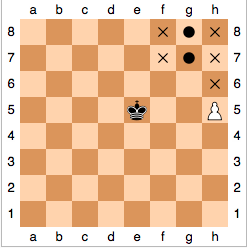
\includegraphics{keysquares.png}
\caption{Critical squares for the white king to reach.}
\label{fig:keysquares}
\end{figure}
This strategy would work in more cases than the one described in section
\ref{sec:strategy}, because there are situations where \wk can reach one of those squares in time, but
not get directly next to \wp. The disadvantage is that is much more complicated, since there are now
more options for \bk to interfere with \wk's movement.

\section{Testing}


\end{document}






















